\documentclass{article}
\usepackage[landscape, margin=5mm, paper=a5paper, includehead, includefoot]{geometry}
\usepackage{lipsum}
\usepackage{graphicx}
\usepackage{multicol}
\usepackage{fancyhdr}
\usepackage{scrextend}
\usepackage{paralist}

\KOMAoptions{fontsize=8pt}
\setlength{\parindent}{0pt}
\raggedright

% Define fancy headers and footers
\pagestyle{fancy}
\fancyhf{}
\fancyhead[L]{\leftmark}
\fancyfoot[C]{\thepage}


%%%%%%%%%%%%% DOCUMENT START %%%%%%%%%%%%%
\begin{document}
\pagenumbering{gobble}

%%%%%%%%%%%%%%%%%% KUPFERLEGIERUNG %%%%%%%%%%%%%%%%%%%%%%
\newpage
% HEADER:
\pagestyle{fancy}
\fancyhf{}
\fancyhead[L]{GMT}
\fancyhead[C]{Werkstoffe-Main}
\fancyhead[R]{Kupferlegierung}

%\vspace{-10mm}
\begin{multicols}{3}

\paragraph{Kupferlegierung:}

\includegraphics[width=\linewidth]{copper.jpg}
\paragraph{Allgemeine Informaionen} Dichte: Die Dichte von Kupferlegierungen
variiert je nach Legierung und beträgt im Allgemeinen zwischen 7,7 und 8,8 $\frac{g}{cm^3}$.

Zugfestigkeit: Die Zugfestigkeit von Kupferlegierungen hängt von der genauen
Legierung ab. Beispielsweise hat eine typische Messinglegierung eine
Zugfestigkeit von etwa 350 MPa.

Aus was ist es hergestellt? Kupferlegierungen werden aus einer Mischung von
Kupfer und anderen Metallen hergestellt, um bestimmte Eigenschaften wie Härte,
Festigkeit, Korrosionsbeständigkeit und elektrische Leitfähigkeit zu erzielen.
Beispiele für Kupferlegierungen sind Messing (Kupfer und Zink), Bronze (Kupfer
und Zinn) und Kupfer-Nickel-Legierungen.

Wie ist es hergestellt? Kupferlegierungen werden durch Schmelzen der
Ausgangsmetalle und Mischen in einem Ofen hergestellt. Die Legierung wird dann
in eine Form gegossen und abgekühlt, um ein fertiges Produkt zu erhalten.

\paragraph{Verwendung:}
Kupferlegierungen werden in einer Vielzahl von Anwendungen eingesetzt,
  darunter Elektrotechnik, Bauwesen, Schmuckherstellung, Automobilindustrie,
  Luft- und Raumfahrtindustrie sowie in der Lebensmittelindustrie.

\paragraph{Verwertung:}
Kupferlegierungen können durch Recycling wiederverwendet werden. Das
  Recycling von Kupferlegierungen spart Energie und Ressourcen im Vergleich zur
  Herstellung von neuen Kupferlegierungen aus Rohstoffen.

\paragraph{Entsorgung:}
Kupferlegierungen können als Altmetall entsorgt werden. Recycling ist
  jedoch die bevorzugte Methode, da es dazu beiträgt, die Umweltauswirkungen zu
  minimieren.

\paragraph{Warum ist es wichtig?}
Kupferlegierungen sind aufgrund ihrer einzigartigen Kombination aus
  Eigenschaften wie Festigkeit, Härte und Korrosionsbeständigkeit in vielen
  Industriezweigen unverzichtbar. Darüber hinaus ist Kupfer eine hervorragende
  elektrische Leitfähigkeit, was es zu einem wichtigen Material in der
  Elektrotechnik macht.

\paragraph{Beispiele}
Beispiele für die Verwendung von Kupferlegierungen sind elektrische Kabel
  und Leitungen, Rohre, Schmuck, Münzen, Armaturen, elektronische Bauteile und
  Turbinen in der Energieerzeugung. Kupferlegierungen werden auch in der
  Medizintechnik eingesetzt, beispielsweise für Implantate und Instrumente. In
  der Bauindustrie werden Kupferlegierungen für Dächer, Fassadenverkleidungen
  und Wasserleitungen verwendet. In der Automobilindustrie werden
  Kupferlegierungen für Bremsleitungen und Kühlsysteme verwendet. In der Luft-
  und Raumfahrtindustrie werden Kupferlegierungen für Strahltriebwerke,
  Raumfahrzeuge und Flugzeuge verwendet.en in der Energieerzeugung.
  Kupferlegierungen werden auch in der Medizintechnik eingesetzt,
  beispielsweise für Implantate und Instrumente. In der Bauindustrie werden
  Kupferlegierungen für Dächer, Fassadenverkleidungen und Wasserleitungen
  verwendet. In der Automobilindustrie werden Kupferlegierungen für
  Bremsleitungen und Kühlsysteme verwendet. In der Luft- und Raumfahrtindustrie
  werden Kupferlegierungen für Strahltriebwerke, Raumfahrzeuge und Flugzeuge
  verwendet.

\end{multicols}
\fancyfoot[L]{Daniel Renschler}
\fancyfoot[R]{J1-2}
\clearpage

%%%%%%%%%%%%%%%%%%%%%%% ELASTOMERE %%%%%%%%%%%%%%%%%%%
\newpage
% HEADER:
\pagestyle{fancy}
\fancyhf{}
\fancyhead[L]{GMT}
\fancyhead[C]{Werkstoffe-Main}
\fancyhead[R]{Elastomere}

%\vspace{-10mm}
\begin{multicols}{3}

\paragraph{Elastomere:}
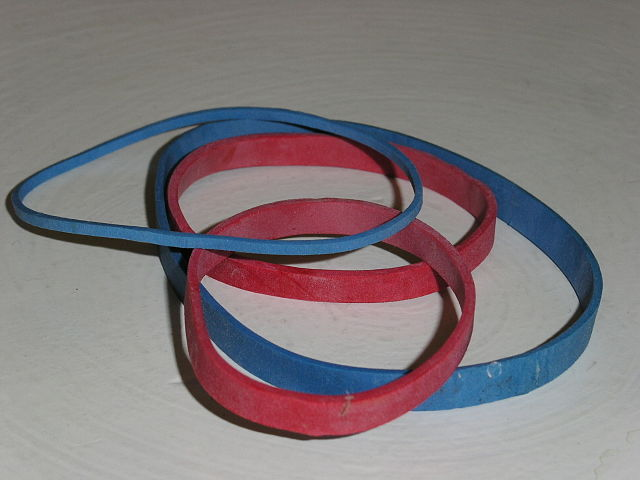
\includegraphics[width=\linewidth]{elasto.jpeg}

\paragraph{Allgemeine Informationen}
Dichte: Die Dichte von Elastomeren variiert, aber liegt normalerweise im Bereich von 0,90 bis 1,20 g/cm$^3$.
Zugfestigkeit: Die Zugfestigkeit von Elastomeren variiert ebenfalls je nach Material und Herstellungsmethode. Typischerweise beträgt sie zwischen 10 und 30 MPa.

Aus was ist es hergestellt?
Elastomere werden aus synthetischen oder natürlichen Polymeren hergestellt. Natürliche Elastomere stammen aus pflanzlichen Quellen, wie z.B. dem Kautschukbaum. Synthetische Elastomere werden aus Erdölprodukten hergestellt.

Wie ist es hergestellt?
Elastomere werden normalerweise durch Polymerisation hergestellt. Dies ist ein chemischer Prozess, bei dem Monomere miteinander reagieren, um lange Ketten von Polymeren zu bilden. Diese Polymerketten sind elastisch und flexibel, was Elastomere zu einem sehr dehnbaren und widerstandsfähigen Material macht.

\paragraph{Verwendung:}
\begin{compactitem}
\item Elastomere werden häufig in der Herstellung von Gummiwaren eingesetzt, wie z.B. Reifen, Schläuchen und Dichtungen.
\item Elastomere werden auch in der Medizin eingesetzt, z.B. in der Herstellung von medizinischen Handschuhen, Kathetern und Blutbeuteln.
\item Elastomere werden auch in der Elektroindustrie eingesetzt, z.B. als Isoliermaterialien für Kabel und Leitungen.
\end{compactitem}

\paragraph{Verwertung:}
\begin{compactitem}
\item Elastomere können recycelt werden, indem sie zerkleinert und zu neuen Produkten verarbeitet werden.
\item Sie können auch als Brennstoff in speziellen Anlagen verbrannt werden.
\end{compactitem}

\paragraph{Entsorgung:}
\begin{compactitem}
\item Elastomere sollten getrennt von anderen Abfallstoffen entsorgt werden.
\item Sie können in speziellen Anlagen verbrannt oder deponiert werden.
\end{compactitem}

\paragraph{Warum ist es wichtig?}
\begin{compactitem}
\item Elastomere sind aufgrund ihrer hohen Elastizität und Flexibilität ein äußerst wichtiges Material in vielen Branchen.
\item Die Verwendung von Elastomeren hat zu zahlreichen Fortschritten in der Technologie beigetragen, z.B. bei der Entwicklung von Reifen, Schläuchen und Dichtungen, die in vielen Bereichen unverzichtbar sind.
\end{compactitem}

\paragraph{Beispiele}
\begin{compactitem}
\item Reifen für Fahrzeuge
\item Dichtungen für Rohre und Behälter
\item Schläuche für die Medizin
\end{compactitem}
\paragraph{Zusammenfassung:} Elastomere sind gummiartige Werkstoffe mit hoher Dehnbarkeit und Rückstellkräften, die für Anwendungen wie Dichtungen, Schläuche, Gummibänder und Reifen verwendet werden.


\end{multicols}

\fancyfoot[L]{Daniel Renschler}
\fancyfoot[R]{J1-2}
\clearpage


%%%%%%%%%%%%%%%%%%%%%%%%% HOLZWERKSTOFFE %%%%%%%%%%%%%%%%%%%%%%%%
\newpage
% HEADER:
\pagestyle{fancy}
\fancyhf{}
\fancyhead[L]{GMT}
\fancyhead[C]{Werkstoffe-Main}
\fancyhead[R]{Holzwerkstoffe}

%\vspace{-10mm}
\begin{multicols}{3}

\paragraph{Holzwerkstoffe:}

\includegraphics[width=\linewidth]{osb.jpg}

\paragraph{Allgemeine Informationen:}
Die Dichte von Holzwerkstoffen variiert je nach Art des Holzwerkstoffs und
seiner Herstellung. Zum Beispiel beträgt die Dichte von Spanplatten etwa
600-800 kg/m³, während die Dichte von OSB-Platten (Oriented Strand Board) je
nach Dicke und Ausrichtung der Schichten zwischen 550 und 800 kg/m³ liegt.

Die Zugfestigkeit von Holzwerkstoffen hängt ebenfalls von der Art des
Werkstoffs und seiner Herstellung ab. Zum Beispiel beträgt die Zugfestigkeit
von Spanplatten etwa 0,2-0,4 N/mm², während die Zugfestigkeit von OSB-Platten
je nach Dicke und Ausrichtung der Schichten zwischen 0,5 und 1,5 N/mm² liegt.

Holzwerkstoffe werden aus Holz oder Holzresten hergestellt, die zu Holzspänen,
Holzfasern oder Holzschichten zerkleinert werden. Diese werden dann mit
Bindemitteln wie Leim oder Harz zu Platten, Brettern oder anderen Formen
verarbeitet.

\paragraph{Verwendung:}
Holzwerkstoffe werden in vielen Anwendungen verwendet, zum Beispiel in der
Möbelherstellung, im Innenausbau, im Bauwesen und in der Verpackungsindustrie.
Sie können auch für dekorative Zwecke eingesetzt werden.

\paragraph{Verwertung:}
Holzwerkstoffe können je nach Art und Herstellung recycelt werden. Zum Beispiel
können Spanplatten in ihre Bestandteile zerlegt und recycelt werden.
OSB-Platten können auch recycelt werden, indem sie zerkleinert und zur
Herstellung neuer Platten wiederverwendet werden.

\paragraph{Entsorgung:}
Holzwerkstoffe können in der Regel wie normales Holz entsorgt werden. Je nach
Art des Holzwerkstoffs und der Verwendung können jedoch zusätzliche Schritte
zur Entsorgung erforderlich sein.

\paragraph{Warum sind sie wichtig?}
Holzwerkstoffe sind wichtig, da sie eine nachhaltige Alternative zu Vollholz
darstellen und viele Vorteile bieten, wie zum Beispiel eine höhere Festigkeit,
Haltbarkeit und Dimensionsstabilität. Sie können auch aus recycelten
Materialien hergestellt werden, was zu einer Verringerung der Umweltbelastung
beiträgt.

\paragraph{Beispiele:}
Einige Beispiele für die Verwendung von Holzwerkstoffen sind:
\begin{compactitem}
  \item Spanplatten für Möbel oder Fußböden
  \item OSB-Platten für Dachdeckungen, Wandverkleidungen oder Unterkonstruktionen
  \item MDF-Platten für Möbel oder Wandverkleidungen
\end{compactitem}

\end{multicols}

\fancyfoot[L]{Daniel Renschler}
\fancyfoot[R]{J1-2}
\clearpage

%%%%%%%%%%%%%%%%%%%%%%%%% ALUMINIUM %%%%%%%%%%%%%%%%%%%%%%%%
\newpage
% HEADER:
\pagestyle{fancy}
\fancyhf{}
\fancyhead[L]{GMT}
\fancyhead[C]{Werkstoffe-Main}
\fancyhead[R]{Aluminium}

%\vspace{-10mm}
\begin{multicols}{3}

\paragraph{Aluminium:}

\includegraphics[width=\linewidth]{alu.jpg}
\paragraph{Allgemeine Informationen}
Dichte: Die Dichte von Aluminium beträgt in der Regel etwa 2,7
g/cm\textsuperscript{3}.
Zugfestigkeit: Die Zugfestigkeit von Aluminium kann je nach Legierung und
Verarbeitung zwischen 50 und 700 N/mm\textsuperscript{2} liegen.

Aus was ist es hergestellt?
Aluminium wird aus dem Erz Bauxit gewonnen. Zunächst wird das Erz zu
Aluminiumoxid verarbeitet, das dann durch Schmelzen und Elektrolyse in
Aluminium umgewandelt wird.

Wie ist es hergestellt?
Die Herstellung von Aluminium beginnt mit dem Abbau von Bauxit. Das Bauxit wird
zerkleinert, gewaschen und zu Aluminiumoxid verarbeitet. Das Aluminiumoxid wird
dann in einem Schmelzofen geschmolzen und durch Elektrolyse in Aluminium
umgewandelt.

\paragraph{Verwendung:}
\begin{compactitem}
\item Aluminium wird oft als Konstruktionsmaterial verwendet, z.B. in
  Flugzeugen, Autos, Gebäuden und Brücken.
\item Es wird auch in der Verpackungsindustrie eingesetzt, z.B. für
  Getränkedosen.
\item Aluminium wird auch für elektronische Anwendungen verwendet, z.B. als
  Leiterplatte in Computern und anderen Geräten.
\end{compactitem}

\paragraph{Verwertung:}
\begin{compactitem}
\item Aluminium kann recycelt werden und ist zu 100\% wiederverwendbar. Das
  Recycling von Aluminium spart Energie und Ressourcen und reduziert die Menge
  an Abfall, die auf Deponien landet.
\item Das Recycling von Aluminium erfordert nur etwa 5\% der Energie, die für
  die Herstellung von neuem Aluminium benötigt wird.
\end{compactitem}

\paragraph{Entsorgung:}
\begin{compactitem}
\item Aluminium kann auf Deponien entsorgt werden, wo es sich aufgrund seiner
  hohen Beständigkeit gegen Korrosion und Oxidation nicht zersetzt.
\item Recycling ist jedoch die bevorzugte Methode zur Entsorgung von Aluminium,
  da es wiederverwendbar ist und die Umweltbelastung reduziert.
\end{compactitem}

\paragraph{Warum ist es wichtig?}
\begin{compactitem}
\item Aluminium ist aufgrund seiner hohen Festigkeit, seines geringen Gewichts
  und seiner Beständigkeit gegen Korrosion und Oxidation ein vielseitiger
  Werkstoff, der in vielen Branchen eingesetzt wird.
\item Das Recycling von Aluminium spart Energie und Ressourcen und reduziert die Menge an Abfall, die auf Deponien landet.
\end{compactitem}

\paragraph{Beispiele}
Beispiele für die Verwendung von Aluminium sind: Flugzeugbau, Automobilbau,
Bauwesen, Verpackungsindustrie und Elektronik.
\end{multicols}

\fancyfoot[L]{Daniel Renschler}
\fancyfoot[R]{J1-2}
\clearpage

%%%%%%%%%%%%%% STAHL %%%%%%%%%%%%%%%%%%%%%%%
\newpage
% HEADER:
\pagestyle{fancy}
\fancyhf{}
\fancyhead[L]{GMT}
\fancyhead[C]{Werkstoffe-Main}
\fancyhead[R]{Stahl}

\begin{multicols}{3}

\paragraph{Stahl:}
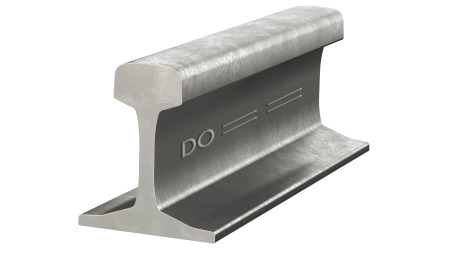
\includegraphics[width=\linewidth]{stahl.jpg}
\paragraph{Allgemeine Informationen}
Dichte: Die Dichte von Stahl beträgt etwa 7,85 g/cm$^3$. Zugfestigkeit: Die
Zugfestigkeit von Stahl variiert je nach Legierung und Wärmebehandlung, kann
jedoch bis zu 2000 N/mm$^2$ erreichen.

Aus was ist es hergestellt? Stahl ist eine Legierung aus Eisen und Kohlenstoff,
wobei der Kohlenstoffanteil je nach Legierung zwischen 0,2\% und 2,1\% liegen
kann.

Wie ist es hergestellt? Stahl wird in einem Hochofen aus Eisenerz und Koks
hergestellt. Der Kohlenstoff im Koks bindet den Sauerstoff im Eisenerz und
bildet Kohlenmonoxid, das als Reduktionsmittel dient. Die so erzeugte flüssige
Roheisen wird dann in einem Konverter von unerwünschten Verunreinigungen
befreit und in Stahl umgewandelt.

\paragraph{Verwendung:}
\begin{compactitem}
\item Stahl wird in der Bauindustrie für Träger, Balken und Stützen verwendet,
  da es sehr stark und langlebig ist.
\item Auch in der Automobilindustrie findet Stahl Anwendung, insbesondere für
  Karosserie- und Chassiskomponenten.
\item Aufgrund seiner Beständigkeit gegen Korrosion wird Edelstahl für
  Küchengeräte und medizinische Instrumente verwendet.
\end{compactitem}

\paragraph{Verwertung:}
\begin{compactitem}
\item Stahl kann durch Schmelzen recycelt werden, um neues Metall herzustellen.
\item Es gibt auch Prozesse zur Wiederverwendung von Stahlprodukten, wie zum
  Beispiel die Verwendung von gebrauchten Stahlträgern in neuen Gebäuden.
\end{compactitem}

\paragraph{Entsorgung:}
\begin{compactitem}
\item Stahl kann recycelt werden, was eine umweltfreundliche und kostengünstige
  Entsorgungsmethode darstellt.
\item Es ist auch möglich, Stahl auf Deponien zu entsorgen, aber dies kann
  aufgrund des Platzbedarfs und der begrenzten Verfügbarkeit von Deponieraum
  problematisch sein.
\end{compactitem}

\paragraph{Warum ist es wichtig?}
\begin{compactitem}
\item Stahl ist aufgrund seiner Festigkeit, Haltbarkeit und Vielseitigkeit ein
  wichtiger Werkstoff in vielen Branchen und Anwendungen.
\item Stahl ist auch relativ kostengünstig im Vergleich zu anderen Materialien,
  was dazu beiträgt, dass es weit verbreitet ist und in vielen Ländern ein
  wichtiger Wirtschaftszweig ist.
\item Die Recyclingfähigkeit von Stahl macht es zu einer nachhaltigen Option
  für die Industrie.
\end{compactitem}

\paragraph{Beispiele}
Stahl wird in vielen Bereichen der Industrie eingesetzt, wie zum Beispiel
  im Bauwesen für Träger und Stützen, im Maschinen- und Fahrzeugbau für
  Karosserien und Motorteile, in der Verpackungsindustrie für Dosen und
  Behälter, sowie in der Energieerzeugung für Turbinen und Generatoren.

\paragraph{Zusammenfassung}
Stahl ist ein vielseitiger und wichtiger Werkstoff für die Industrie aufgrund
seiner hohen Festigkeit, Haltbarkeit und Korrosionsbeständigkeit.Stahl ist auch eine nachhaltige
Option, da es recycelbar ist und somit die Umweltbelastung reduziert.
\end{multicols}

\fancyfoot[L]{Daniel Renschler}
\fancyfoot[R]{J1-2}
\clearpage

%%%%%%%%%MASSIVHOLZ%%%%%%%%%%%
\newpage
% HEADER:
\pagestyle{fancy}
\fancyhf{}
\fancyhead[L]{GMT}
\fancyhead[C]{Werkstoffe-Main}
\fancyhead[R]{Massivholz}

%\vspace{-10mm}
\begin{multicols}{3}

\paragraph{Massivholz:}
\includegraphics[width=\linewidth]{Holz.jpg}

\paragraph{Allgemeine Informationen}
Dichte: Die Dichte von Massivholz variiert
je nach Baumart und Feuchtigkeitsgehalt. Sie kann zwischen 300 und 1000
kg/m$^3$ liegen. Zugfestigkeit: Die Zugfestigkeit variiert auch je nach Baumart
und Feuchtigkeitsgehalt, sie liegt jedoch meist im Bereich von 30 bis 90
N/mm$^2$.

Aus was ist es hergestellt? Massivholz wird aus Bäumen hergestellt, die gefällt
und zu Holzplanken verarbeitet werden.

Wie ist es hergestellt? Die Herstellung von Massivholz beginnt mit der Fällung
von Bäumen. Das Holz wird dann zugeschnitten, getrocknet und zu Planken
verarbeitet. Es gibt verschiedene Verarbeitungsmethoden, darunter Sägen, Hobeln
und Schleifen.

\paragraph{Verwendung:}
Massivholz wird in der Möbelherstellung, im Bauwesen und in der Herstellung von
dekorativen Gegenständen wie Bilderrahmen verwendet.

\paragraph{Verwertung:}
Massivholz kann wiederverwendet werden, beispielsweise durch den Bau von Möbeln
oder Holzhäusern. Es kann auch in der Papierherstellung recycelt werden.

\paragraph{Entsorgung:}
Massivholz kann auf verschiedene Weise entsorgt werden, darunter durch
Kompostierung, Verbrennung oder Deponierung. Kompostierung ist die bevorzugte
Methode, da es zur Bodenverbesserung beiträgt.

\paragraph{Warum ist es wichtig?}
Massivholz ist ein nachwachsender Rohstoff, der in der Bau- und Möbelindustrie
weit verbreitet ist. Es ist eine nachhaltige Option, da es bei sachgemäßer
Bewirtschaftung immer wieder nachwachsen kann.

\paragraph{Beispiele}
Beispiele für die Verwendung von Massivholz sind Parkettböden, Möbel wie
Tische, Stühle und Betten sowie Balken und Rahmen im Hausbau.

\paragraph{Zusammenfassung}
\begin{compactitem}
  \item Massivholz wird aus natürlichen Baumstämmen geschnitten und ist ein
    traditioneller und bewährter Werkstoff in vielen Bereichen.
  \item Es ist ein erneuerbarer Rohstoff, da Holz nachwächst und Bäume
    nachhaltig angebaut werden können.
  \item Aufgrund seiner natürlichen Eigenschaften ist Massivholz atmungsaktiv
    und kann die Luftfeuchtigkeit in einem Raum regulieren.
  \item Massivholz kann für eine Vielzahl von Anwendungen verwendet werden, wie
    z.B. für Möbel, Bodenbeläge, Wandverkleidungen, Bauteile in der
    Bauindustrie und vieles mehr.
  \item Wenn Massivholz nicht mehr benötigt wird, kann es entweder recycelt
    oder biologisch abgebaut werden. Holzabfälle können auch als Brennstoffe
    oder Rohstoffe für andere Produkte verwendet werden.
\end{compactitem}



\end{multicols}

\fancyfoot[L]{Daniel Renschler}
\fancyfoot[R]{J1-2}
\clearpage

%%%%%%%% DUROMERE %%%%%%%%%%%%%
\newpage
% HEADER:
\pagestyle{fancy}
\fancyhf{}
\fancyhead[L]{GMT}
\fancyhead[C]{Werkstoffe-Main}
\fancyhead[R]{Duromere}

\begin{multicols}{3}

\paragraph{Duromere:}
\includegraphics[width=\linewidth]{duroplaste.png}
\paragraph{Allgemeine Informationen}
Dichte: Die Dichte von Duromeren variiert je nach Art und kann zwischen 1,2 und
2,0 g/cm$^3$ liegen.
Zugfestigkeit: Die Zugfestigkeit von Duromeren hängt ebenfalls von der Art ab
und kann zwischen 40 und 200 N/mm$^2$ liegen.

\textbf{Aus was ist es hergestellt?}
Duromere werden durch Polymerisation von Monomeren hergestellt, die in der
Regel aus Erdöl gewonnen werden. Das Polymerisationsverfahren führt zu einem
festen, nicht schmelzbaren Kunststoff, der in der Regel duroplastisch ist, d.h.
nach der Aushärtung nicht mehr verformbar.

\textbf{Wie ist es hergestellt?}
Die Herstellung von Duromeren erfolgt durch Polymerisation von Monomeren,
entweder durch Wärmebehandlung oder durch den Einsatz von chemischen
Katalysatoren. Der Prozess der Polymerisation führt zur Bildung von Netzwerken,
die eine dreidimensionale Struktur bilden und zu einer Erhöhung der Festigkeit
und Steifigkeit des Kunststoffs führen.

\paragraph{Verwendung:}
Duromere werden aufgrund ihrer hohen Festigkeit, Steifigkeit und
Temperaturbeständigkeit in einer Vielzahl von Anwendungen eingesetzt, z.B. in
der Automobilindustrie, Luftfahrt, Elektronik, Bauindustrie, medizinischen
Geräten und Sportgeräten.

\paragraph{Verwertung:}
Duromere können nicht recycelt werden und werden in der Regel verbrannt, um
Energie zurückzugewinnen.

\paragraph{Entsorgung:}
Die Entsorgung von Duromeren erfolgt in der Regel durch Verbrennung, wobei es
zu Freisetzung von Kohlenstoffdioxid und anderen Schadstoffen kommen kann.

\paragraph{Warum ist es wichtig?}
Duromere sind aufgrund ihrer hohen Festigkeit und Steifigkeit ein wichtiger
Werkstoff in vielen Branchen, insbesondere in der Automobil- und
Luftfahrtindustrie, wo sie dazu beitragen, Gewicht und Emissionen zu
reduzieren. Sie bieten auch eine hohe Beständigkeit gegenüber chemischen
Angriffen und hohen Temperaturen.

\paragraph{Beispiele}
Beispiele für die Verwendung von Duromeren sind: Gehäuse von elektronischen
Geräten, Luft- und Raumfahrtbauteile, Karosserieteile von Autos, Rohre,
medizinische Geräte, Sportausrüstung und Baukomponenten.

\paragraph{Zusammenfassung}
Duromere sind Polymerwerkstoffe, die sich durch hohe Festigkeit, Härte und
Steifigkeit auszeichnen. Sie bestehen aus einer vernetzten Polymermatrix, die
durch chemische Reaktionen aushärtet. Die Dichte, Zugfestigkeit und
Herstellungsmethoden können je nach Typ und Anwendung variieren. Duromere
werden in einer Vielzahl von Produkten eingesetzt, wie z.B. in Gehäusen,
Elektrogeräten, Automobilteilen, und medizinischen Implantaten.

\end{multicols}

\fancyfoot[L]{Daniel Renschler}
\fancyfoot[R]{J1-2}
\clearpage


\newpage
% HEADER:
\pagestyle{fancy}
\fancyhf{}
\fancyhead[L]{GMT}
\fancyhead[C]{Werkstoffe-Main}
\fancyhead[R]{Thermoplaste}

%\vspace{-10mm}
\begin{multicols}{3}

\paragraph{Thermoplaste:}
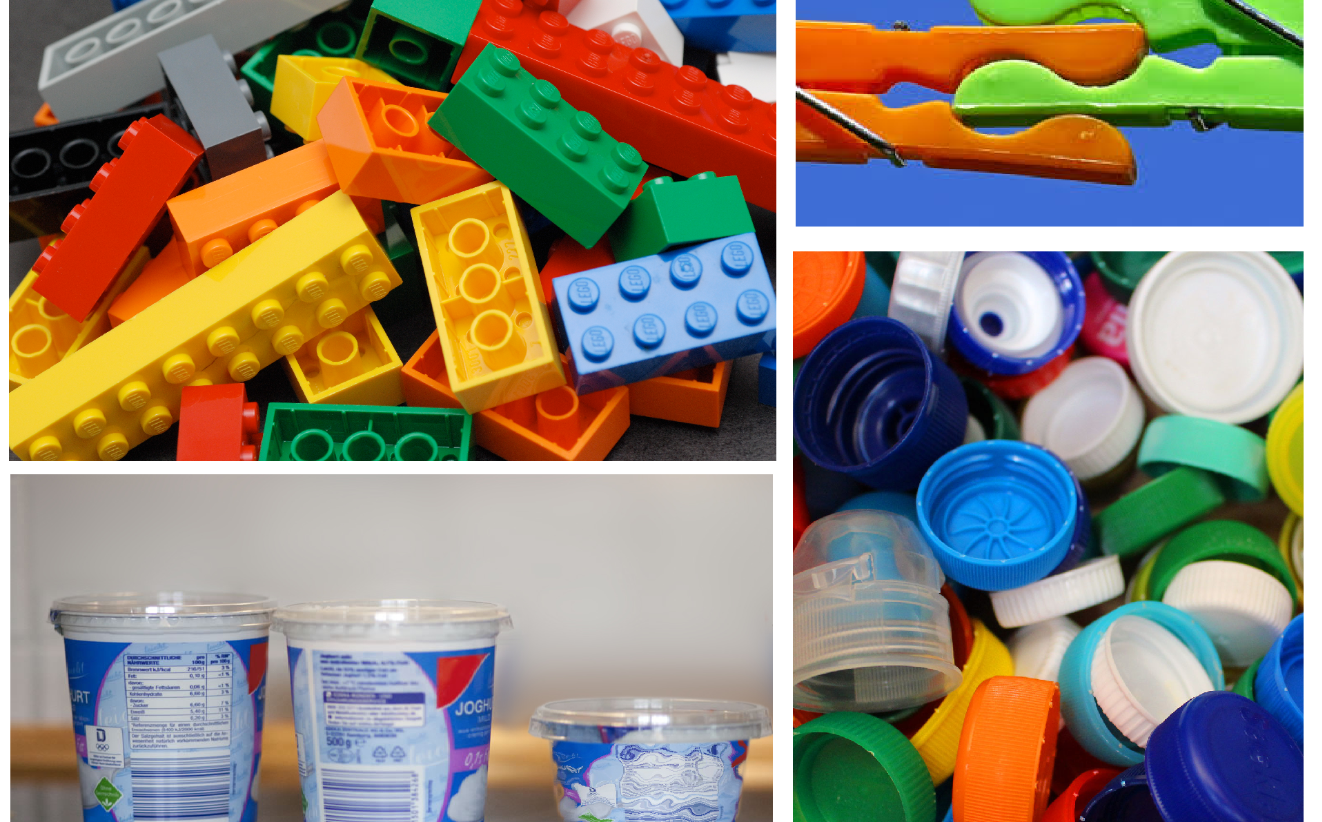
\includegraphics[width=\linewidth]{thermoplast.png}
\paragraph{Allgemeine Informationen}
Dichte: Die Dichte von Thermoplasten variiert stark je nach Materialtyp,
Herstellung und Form. Sie kann zwischen 0,8 und 2,3 g/cm\textsuperscript{3}
liegen.

Zugfestigkeit: Die Zugfestigkeit von Thermoplasten variiert ebenfalls je nach
Materialtyp und kann zwischen 20 und 70 N/mm\textsuperscript{2} liegen.

Aus was ist es hergestellt? Thermoplaste bestehen aus Polymeren, die aus
monomeren Einheiten durch Polymerisation hergestellt werden.

Wie ist es hergestellt? Thermoplaste werden in einem Polymerisationsprozess
hergestellt, bei dem Monomere unter Einwirkung von Wärme und/oder Druck zu
Polymeren reagieren.

\paragraph{Verwendung:}
Thermoplaste werden in einer Vielzahl von Anwendungen eingesetzt, insbesondere
in der Kunststoffindustrie, aber auch in der Verpackungs-, Automobil- und
Elektronikindustrie.

\paragraph{Verwertung:}
Thermoplaste können recycelt werden, indem sie geschmolzen und in neue Produkte
umgewandelt werden. Aufgrund der hohen Sortenreinheit und der guten
Reproduzierbarkeit eignen sie sich gut für das Recycling.

\paragraph{Entsorgung:}
Thermoplaste können auf Deponien entsorgt werden, aber aufgrund ihrer
Recyclingfähigkeit ist dies nicht die beste Option. Die Verbrennung von
Thermoplasten zur Energiegewinnung ist ebenfalls möglich, sollte jedoch
vermieden werden, um die Menge an Treibhausgasemissionen zu reduzieren.

\paragraph{Warum ist es wichtig?}
Thermoplaste sind aufgrund ihrer Vielseitigkeit und ihrer Recyclingfähigkeit
ein wichtiger Werkstoff für eine nachhaltige Wirtschaft. Sie können dazu
beitragen, den Verbrauch von nicht erneuerbaren Ressourcen zu reduzieren und
die Menge an Abfällen zu verringern.

\paragraph{Beispiele}
Beispiele für die Verwendung von Thermoplasten sind PET-Flaschen, PVC-Rohre,
Nylon-Fasern, Polyethylen-Folien und Polycarbonat-Brillengläser.

\paragraph{Beispiele}
Thermoplaste sind eine Klasse von Kunststoffen, die bei Erhitzung weich und
formbar werden. Sie sind aus linearen oder verzweigten Polymerketten aufgebaut,
die durch schwache Bindungen miteinander verbunden sind. Diese Bindungen
brechen bei Erhitzung auf, wodurch der Kunststoff verformbar wird. Wenn der
Kunststoff abkühlt, werden die Bindungen wiederhergestellt und der Kunststoff
wird wieder fest. Thermoplaste haben eine niedrige Dichte, sind formbar, haben
eine hohe chemische Beständigkeit und sind recycelbar.

Thermoplaste finden in vielen verschiedenen Bereichen Anwendung, wie zum
Beispiel in der Verpackungsindustrie, der Automobilindustrie, der Medizin- und
Elektronikindustrie sowie im Baugewerbe. Einige Beispiele für thermoplastische
Kunststoffe sind Polyethylen, Polypropylen, PVC, Polystyrol und Nylon.
\end{multicols}

\fancyfoot[L]{Daniel Renschler}
\fancyfoot[R]{J1-2}
\clearpage

\newpage
% HEADER:
\pagestyle{fancy}
\fancyhf{}
\fancyhead[L]{GMT}
\fancyhead[C]{Werkstoffe-Main}
\fancyhead[R]{Papier \& Pappe}

%\vspace{-10mm}
\begin{multicols}{3}

\paragraph{Papier \& Pappe:}

\includegraphics[width=\linewidth]{papier_pappe.jpg}
\paragraph{Allgemeine Informationen}
Dichte: Die Dichte von Papier und Pappe hängt von der Dicke des Materials ab
und variiert normalerweise zwischen 0,3 und 1,5 g/cm³.
Zugfestigkeit: Die Zugfestigkeit von Papier und Pappe hängt von der Qualität
und Dicke des Materials ab. Sie variiert normalerweise zwischen 20 und 200
N/mm².

Aus was ist es hergestellt? Papier wird in der Regel aus Holzschliff oder
Zellstoff hergestellt. Pappe besteht aus einer Kombination von Papier- und
Zellstofflagen.

Wie ist es hergestellt? Papier wird durch das Vermischen von Holzschliff oder
Zellstoff mit Wasser und Chemikalien hergestellt, um eine Faserbrei zu bilden.
Dieser Brei wird auf eine Siebform gegossen, um das Wasser abzulassen, und dann
getrocknet und gepresst. Pappe wird aus Papierlagen hergestellt, die mit
Klebstoffen zusammengefügt werden.

\paragraph{Verwendung:}
\begin{compactitem}
\item Papier und Pappe werden häufig für Verpackungen, Bücher, Zeitschriften,
  Druckerpapier und Schreibwaren verwendet.
\item Papier und Pappe können auch für künstlerische Zwecke wie Malerei,
  Collagen und Papiermaché verwendet werden.
\end{compactitem}

\paragraph{Verwertung:}
\begin{compactitem}
\item Papier und Pappe können recycelt werden und werden häufig zu neuen
  Papier- und Kartonprodukten recycelt.
\item Altpapier wird gesammelt, sortiert und verarbeitet, um daraus
  Recyclingpapier und -pappe herzustellen.
\end{compactitem}

\paragraph{Entsorgung:}
\begin{compactitem}
\item Papier und Pappe können auch einfach kompostiert werden.
\item Wenn sie nicht recycelt oder kompostiert werden können, können sie als
  Abfall entsorgt werden.
\end{compactitem}

\paragraph{Warum ist es wichtig?}
\begin{compactitem}
\item Papier und Pappe sind weit verbreitete und vielseitige Materialien, die
  in vielen Bereichen des täglichen Lebens eingesetzt werden.
\item Durch das Recycling von Papier und Pappe können Ressourcen und Energie
  eingespart werden, die zur Herstellung neuer Produkte benötigt werden.
\end{compactitem}

\paragraph{Beispiele}
\begin{compactitem}
\item Verpackungen für Lebensmittel, Medikamente, Elektronik und andere
  Produkte
\item Bücher, Zeitschriften, Druckerpapier und Schreibwaren
\item Isoliermaterialien und Dämmstoffe in der Bauindustrie: Papier und Pappe
  eignen sich aufgrund ihrer geringen Wärmeleitfähigkeit gut als
  Isoliermaterialien und Dämmstoffe in der Bauindustrie. Sie werden zum
  Beispiel als Dämmung für Wände, Dächer und Böden verwendet.
\item Verpackungsmaterial: Aufgrund ihrer Stabilität und Festigkeit werden
  Papier und Pappe häufig als Verpackungsmaterial eingesetzt. Sie werden zum
  Beispiel für Pappkartons, Tragetaschen, Umverpackungen und Versandtaschen
  verwendet.
\end{compactitem}
\end{multicols}

\fancyfoot[L]{Daniel Renschler}
\fancyfoot[R]{J1-2}
\clearpage
%%%%%%%%%%%%%%%%%%% GLAS %%%%%%%%%%%%%%%%%%%

\newpage
% HEADER:
\pagestyle{fancy}
\fancyhf{}
\fancyhead[L]{GMT}
\fancyhead[C]{Werkstoffe-Main}
\fancyhead[R]{Glas}

%\vspace{-10mm}
\begin{multicols}{3}

\paragraph{Glas:}
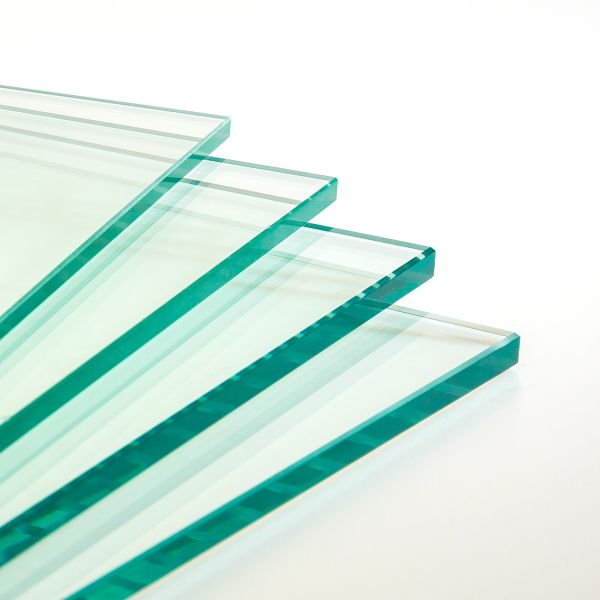
\includegraphics[width=.9\linewidth]{glas.jpg}

\paragraph{Allgemeine Informationen}
Dichte: Die Dichte von Glas hängt von der Art des Glases ab, kann jedoch
zwischen 2,2 und 8 g/cm$^3$ liegen. Zugfestigkeit: Die Zugfestigkeit von Glas
variiert auch je nach Art des Glases und kann zwischen 30 und 200 MPa liegen.

Aus was ist es hergestellt? Glas besteht hauptsächlich aus Siliciumdioxid
(SiO$_2$) sowie anderen anorganischen Verbindungen.

Wie ist es hergestellt? Glas wird hergestellt, indem eine Mischung aus Sand,
Soda und Kalk bei hohen Temperaturen geschmolzen und anschließend abgekühlt
wird.

\paragraph{Verwendung:}
Glas wird häufig für Fenster, Flaschen, Geschirr, optische Linsen,
Laborausrüstung, Leuchten und Schmuck verwendet.

\paragraph{Verwertung:}
Glas kann recycelt werden, indem es eingeschmolzen und zu neuen Glasprodukten
geformt wird.

\paragraph{Entsorgung:}
Glas kann in speziellen Containern oder Recyclingbehältern entsorgt werden, wo
es recycelt oder auf Deponien gelagert werden kann.

\paragraph{Warum ist es wichtig?}
Glas ist ein vielseitiger Werkstoff, der aufgrund seiner Transparenz, Härte und
chemischen Beständigkeit in vielen Anwendungen verwendet wird.

\paragraph{Beispiele}
Beispiele für die Verwendung von Glas sind Fensterscheiben, Flaschen,
Laborgeräte, Smartphone-Displays, Schmuck und Leuchten.

\paragraph{Zusammenfassung}
Glas ist ein spröder, amorpher Feststoff, der durch Abkühlung einer Schmelze
ohne Kristallisation gebildet wird und hauptsächlich aus Siliciumdioxid (SiO$_2$)
besteht. Es hat eine hohe Lichtdurchlässigkeit, chemische Beständigkeit und
kann in verschiedenen Formen wie flach, gebogen oder geblasen hergestellt
werden. Glas findet Verwendung in einer Vielzahl von Anwendungen wie Fenstern,
Geschirr, optischen Linsen, Beleuchtung und als Verpackungsmaterial.
Glas ist ein amorpher, nicht-kristalliner Feststoff, der aus einer Schmelze
hergestellt wird und häufig in der Bauindustrie, für Fenster und als
Verpackungsmaterial eingesetzt wird. Es hat eine hohe Transparenz, Härte und
chemische Beständigkeit, aber auch eine geringe Bruchfestigkeit.
\end{multicols}

\fancyfoot[L]{Daniel Renschler}
\fancyfoot[R]{J1-2}
\clearpage

\end{document}
